 \section{Methodology}\label{sec:methodology}
We analyzed a year's worth of BGP RIB data and classified instances where we saw multiple ASes announcing the same BGP prefix. We analyzed the BGP data from [.... select a data] in the hopes of identifying a few BGP hijacks. The known BGP hijacks  of this time were [..... list a few hijacks]which our method successfully  identifies. \\
The goal of this study was to understand the frequency and the duration of censorship intended or malicious BGP hijacks. In addition, we  use our data and our understanding of current socio-political situation surrounding the hijack to understand the popular motives behind BGP hijacks. Towards the end, based on our analysis of how most of the hijacks were accomplished, we recommend possible solutions to prevent accidental and malicious BGP hijacks. 
\subsection{Identifying BGP Hijack}
Identifying BGP hijacks involved a carefully filtering RIB table records. 
\begin{enumerate}
\item To identify the instances of BGP hijack, we started out by identifying the instances where we saw two different ASes announcing the same BGP prefix/es.
\item We used a python script to compare the whois records of the ASes announcing the same prefix. If the whois records indicated that the ASNs belonged to the same organization, we ruled out the instance. Large CDNs own many ASes throughout the world. CDNs may announce the same prefix in different parts of the world for traffic engineering. The hope is that the established peering arrangements lead to clients being directed to the closest CDN cache.
\item If the ASes annoucing the same prefix do not belong to the same organization, we check if they have a peering or a customer provider relationship.   We used ... DB to check the relationship between the two ASes[... need to find a tool to use]. This idea of using business relationship was inspired by OpenDNS's classification of BGP \cite{opendns_blackhat_2015}. It is likely that ASes with business relationships might have cosentually borrowed prefixes from teach other.  
\item If we find that the two ASes do not have either peer-peer or customer-provider relation, we then check the geolocation of the two ASes. We make use of the whois record again to compare the geolocation. If the geolocation do not match, then we say we have identified a hijack. 
\item We use bgpstream twitter feed as the `ground truth'. 
\end{enumerate}
 \begin{figure}[!htbp]
	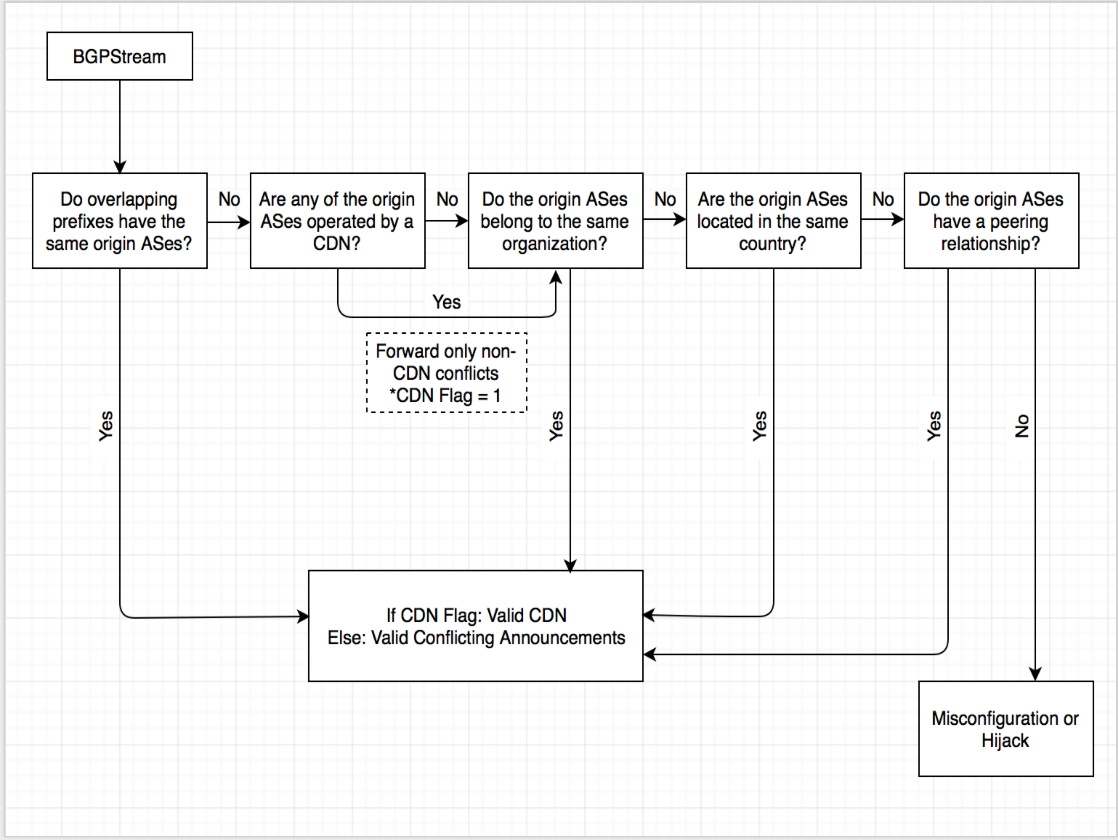
\includegraphics[width=0.5\textwidth]{Algorithm_flowchart.png}
	\caption{Flowchart presets our algorithm that characterizes different types of AS-Origin conflicts.}
	\label{a:label}
\end{figure}
\subsection{Hijack Characterization }

Based on the sociopolitical context and other information we have [...what other infor? ], we manually classify into three categories (1)Misconfiguration, (2)Political hijack for Censorship and (3)Malicious non-political hijack. 

We enumerate the specificity and the number of malicious BGP prefix announcement for each hijack. We calculate the difference in the specificity of the prefix announced by the hijacking AS and the hijacked AS. To determine if there is a cross-national involvement in these hijacks, we enumerate the number of malicious AS prefix announcement for each hijack. We study the geographic distributions of each of the malicious ASes.
We also characterize the target ASes of these hijacks. We determine whether the target selected (1)randomly/for fun , (2) for financial motive, (3) political motive .
\subsection{Hijack Duration and frequency}

